\subsection{Identified entities in the proposed solution}
\begin{itemize}
	\item \textbf{Client:} sends requests to the print server. In order to get the desired action done, the client must send with each request a valid username and its correspondent password.
	\item \textbf{Server:} controls the printer and receives all the requests from the clients. For each request, the server must verify that the client is authenticated. In order to do that, information related to the user that asks for a service is requested to the DBMS. If the username and hashed password match with the information stored in the DBMS, the server will execute the user request.
	\item \textbf{Database management system:} stores all the information regarding the users that can make use of the printing service. For each user, the database holds the username, the salt used for hashing the password and the hashed salt and password.\\
		The database model for this laboratory is represented in \textit{Figure \ref{fig:dbmodel}}.
\end{itemize}
\begin{figure}[hb]
	\centering	
	\begin{tikzpicture}[scale=1.2]
	\umlclass[fill=white]{users}{\textbf{id:} integer <PK>}{\textbf{name:} text NOT NULL UNIQUE\\\textbf{salt:} text NOT NULL\\\textbf{password:} text NOT NULL}
\end{tikzpicture}
	\caption{Implemented database model}
	\label{fig:dbmodel}
\end{figure}
\subsection{Print server interface}
For implementing the server, Java Remote Method Invocation (RMI) is used.\\
The interface follows the one described in the laboratory statement. However, as authentication is to be performed for each invocation, the fields \textit{username} and \textit{passwords} are added. \textit{Code \ref{lst:interface}} gathers the print service interface. 
\begin{lstlisting}[language=Java, caption=Print service interface, basicstyle=\scriptsize, label={lst:interface}]
String print(String filename, String printer, String username, String password);
List<String> queue(String username, String password);
String topQueue(int job, String username, String password);
void start(String username, String password);
void stop(String username, String password);
void restart(String username, String password);
String status(String username, String password);
String readConfig(String parameter, String username, String password);
void setConfig(String parameter, String value, String username, String password);
\end{lstlisting}
\subsection{Service architecture}
\textit{Figure \ref{fig:arch}} shows the simplified print service architecture. As depicted, there is no direct communication between users and DBMS.\\
\begin{figure}[hb]
	\centering
	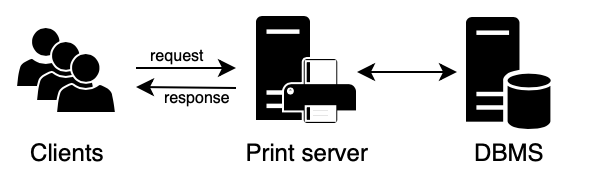
\includegraphics[width=10cm]{images/architecture}
	\caption{Print service architecture}
	\label{fig:arch}
\end{figure}
\\The sequence diagram depicted in \textit{Figure \ref{fig:seqdiag}} explains how the system functions. The client request is only processed if the authentication process successes. Otherwise, the server will respond with a deny of service message.
\begin{figure}[h]
	\centering	
	\begin{tikzpicture}[scale=1.2]
	\begin{umlseqdiag}
		\tikzumlset{font=\scriptsize}
		\umlactor[no ddots, fill=white]{client}
		\umlobject[no ddots, fill=white]{print server}  
		\umldatabase[no ddots, fill=white]{dbms} 
		\begin{umlcall}[op={request,username,password}]{client}{print server}	
			\begin{umlcall}[op={get(username)},return={salt, hash}]{print server}{dbms}	
			\end{umlcall}
			\begin{umlcall}[op={digest=SHA256(salt+password)}]{print server}{print server} 
			\end{umlcall} 
			\begin{umlfragment}[type=alt, label={digest==hash}, inner xsep=15] 
				\begin{umlcall}[op={process request}]{print server}{print server} 
				\end{umlcall} 
				\begin{umlcall}[op={response}]{print server}{client} 
				\end{umlcall} 
				\umlfpart[digest!=hash] 
				\begin{umlcall}[op={access denied}]{print server}{client} 
				\end{umlcall} 
			\end{umlfragment} 
			\end{umlcall}
	\end{umlseqdiag}
\end{tikzpicture}
	\caption{Print service sequence diagram}
	\label{fig:seqdiag}
\end{figure}
\subsection{Print service developed software}
This section summarises all the Java classes developed for this laboratory.\\
For implementing the DBMS, the SQLite database engine has been chosen. The JAR package \textit{sqlite-jdbc} needs to be added to the project before running the code.
\begin{itemize}
	\item \textbf{crypto.HashGenerator:} Java class for generating salts and hashing Strings. The encryption algorithm for hashing the passwords that has been selected is SHA-256. This algorithm, used together with salt, is secure enough for a simple print server.
	\item \textbf{db.DataBaseManager:} Java class for interacting with a SQLite database. User authentication is done in the method \textit{checkUserAuth}. In case there is no prior database, executing its main method a new database will be populated with the users \textit{user1} and \textit{user2}. For simplicity, their passwords will coincide with their username.
	\item \textbf{clientserver.PrintService:} print service interface for RMI application.
	\item \textbf{clientserver.PrintServant:} Java class with all the print services implementation. Before proceeding to execute clients' requests, all the classes will check user authenticity.
	\item \textbf{clientserver.PrintServer:} Java class that implements the RMI server. Run this class for launching the print service.
	\item \textbf{clientserver.Client:} Java class that implements a client. Running this class, the process will prove all the RMI methods, as well as try to access to services with both valid and invalid usernames and passwords.
\end{itemize}